\documentclass[letterpaper,11pt]{article}
\usepackage{setspace} % For double-spaced text
\usepackage{geometry}
\usepackage{multicol}
\usepackage{graphicx}
\usepackage{float}
\usepackage{mathrsfs}

\graphicspath{ {timing_study.png} }
% \doublespacing

\title{CMSE 401 - Homework 4}
\author{Jack Hamel}

\topmargin-2cm     %I recommend adding these three lines to increase the
\textwidth16.5cm   %amount of usable space on the page (and save trees)
\textheight23.5cm
\oddsidemargin0cm

\begin{document}

\maketitle

\section{My Story}

All benchmarking of the codes in this homework were done on dev-intel18 of the HPCC and using the $\texttt{time}$ command to measure runtimes.  I ran the original code with each image provided three times and noted the average runtime; compiling the code with the provided makefile.  Below are the results of this study:
\begin{center}
 \begin{tabular}{|c| c c c c|}
 \hline
 \textbf{Image:} & cube.png & earth.png & MSUStadium.png & sparty.png \\[1.5ex]
 \hline
 \textbf{Time (sec):} & 0.268 & 9.117 & 0.354 & 0.274 \\
 \hline
\end{tabular}
\end{center}
Following this, I tested optimization levels of the GCC compiler.  To do this, I compiled with levels 1-4 and ran the code with the earth.png image.  Below are the results of this study:
\begin{center}
 \begin{tabular}{|c| c c c c|}
 \hline
 \textbf{Optimization Level:} & 1 & 2 & 3 & 4 \\[1.5ex]
 \hline
 \textbf{Time (sec):} & 2.996 & 3.050 & 2.328 & 2.862 \\
 \hline
\end{tabular}
\end{center}
The results of the optimization timing study are interesting for a few reasons.  First, we see no improvement between levels one and two.  Second, level three is faster than level 2 and lastly, which you, the reader, cannot see this, but optimization level four provided the most consistant times.  Every run with level four was within $1ms$ of the average.  

I now began working on improving the performance of the serial (original) code.  To do this, I changed the loop orders of the various filters involved (as the assignment instructed) and ran the code with the cube.png image.  I switched the column and row loop orders for each filter one-by-one and measured the runtime of the code.  After doing so, I noticed no performance improvements.  To remedy this, I decided to submit my test runs using $\texttt{sbatch}$ to hopefully avoid any performance issues caused by running on a dev-node.  After doing so, I still did not notice any performance improvements.  My next step was to use the earth.png image because it requires an order of magntiude more time to run.  I hoped to see more noticeable changes in the performance with a longer runtime.  Now I was beginning to see minute changes in runtimes with each loop order flip.  It was not until I switch the order of the outer loops (loops over r and c) for the gradient, average, and edge thresholding all at once that I finally saw an approximately $7.5\%$ increase in performance in total.  

I now moved onto parallelizing the code with OpenMP.  This was very straightforward.  I simply converted the outermost loop of the average, gradient, and edge thresholding filters to a parallel for loop.  I did not see any situations where this would not work and after comparing the image output to that of the serial code, I confirmed that it was a safe parallelization.  Next, I tested what type of scheduling performs best for my parallel loops.  Since each parallel loop was doing rather similar computations with the same amount/type of input data, I let each loop use the same schedule type at any given time.  I cycled through auto, static, dynamic, and guided scheduling options.  I did not record the performance of each, unfortunately, but I ran each three times while processing earth.png to get a good idea of its speed and guided was the clear winner by $10\%-20\%$.  I then tried setting my chunk size to both 10 and 20, but saw no changes in performance so I decided to not specify a chunk size.  

I then benchmarked the original code, the optimized serial code and my parallel code on the earth.png image. Each time is the average of three runs.  Below are the results of this study:
\begin{center}
 \begin{tabular}{|c| c c c|}
 \hline
 \textbf{Code:} & Original & Optimized & Parallel \\[1.5ex]
 \hline
 \textbf{Time (sec):} & 6.316 & 2.003 & 0.693 \\
 \hline
\end{tabular}
\end{center}
Below is the output image of each code:
\begin{figure}[H]
  \caption{Original Code Earth}
  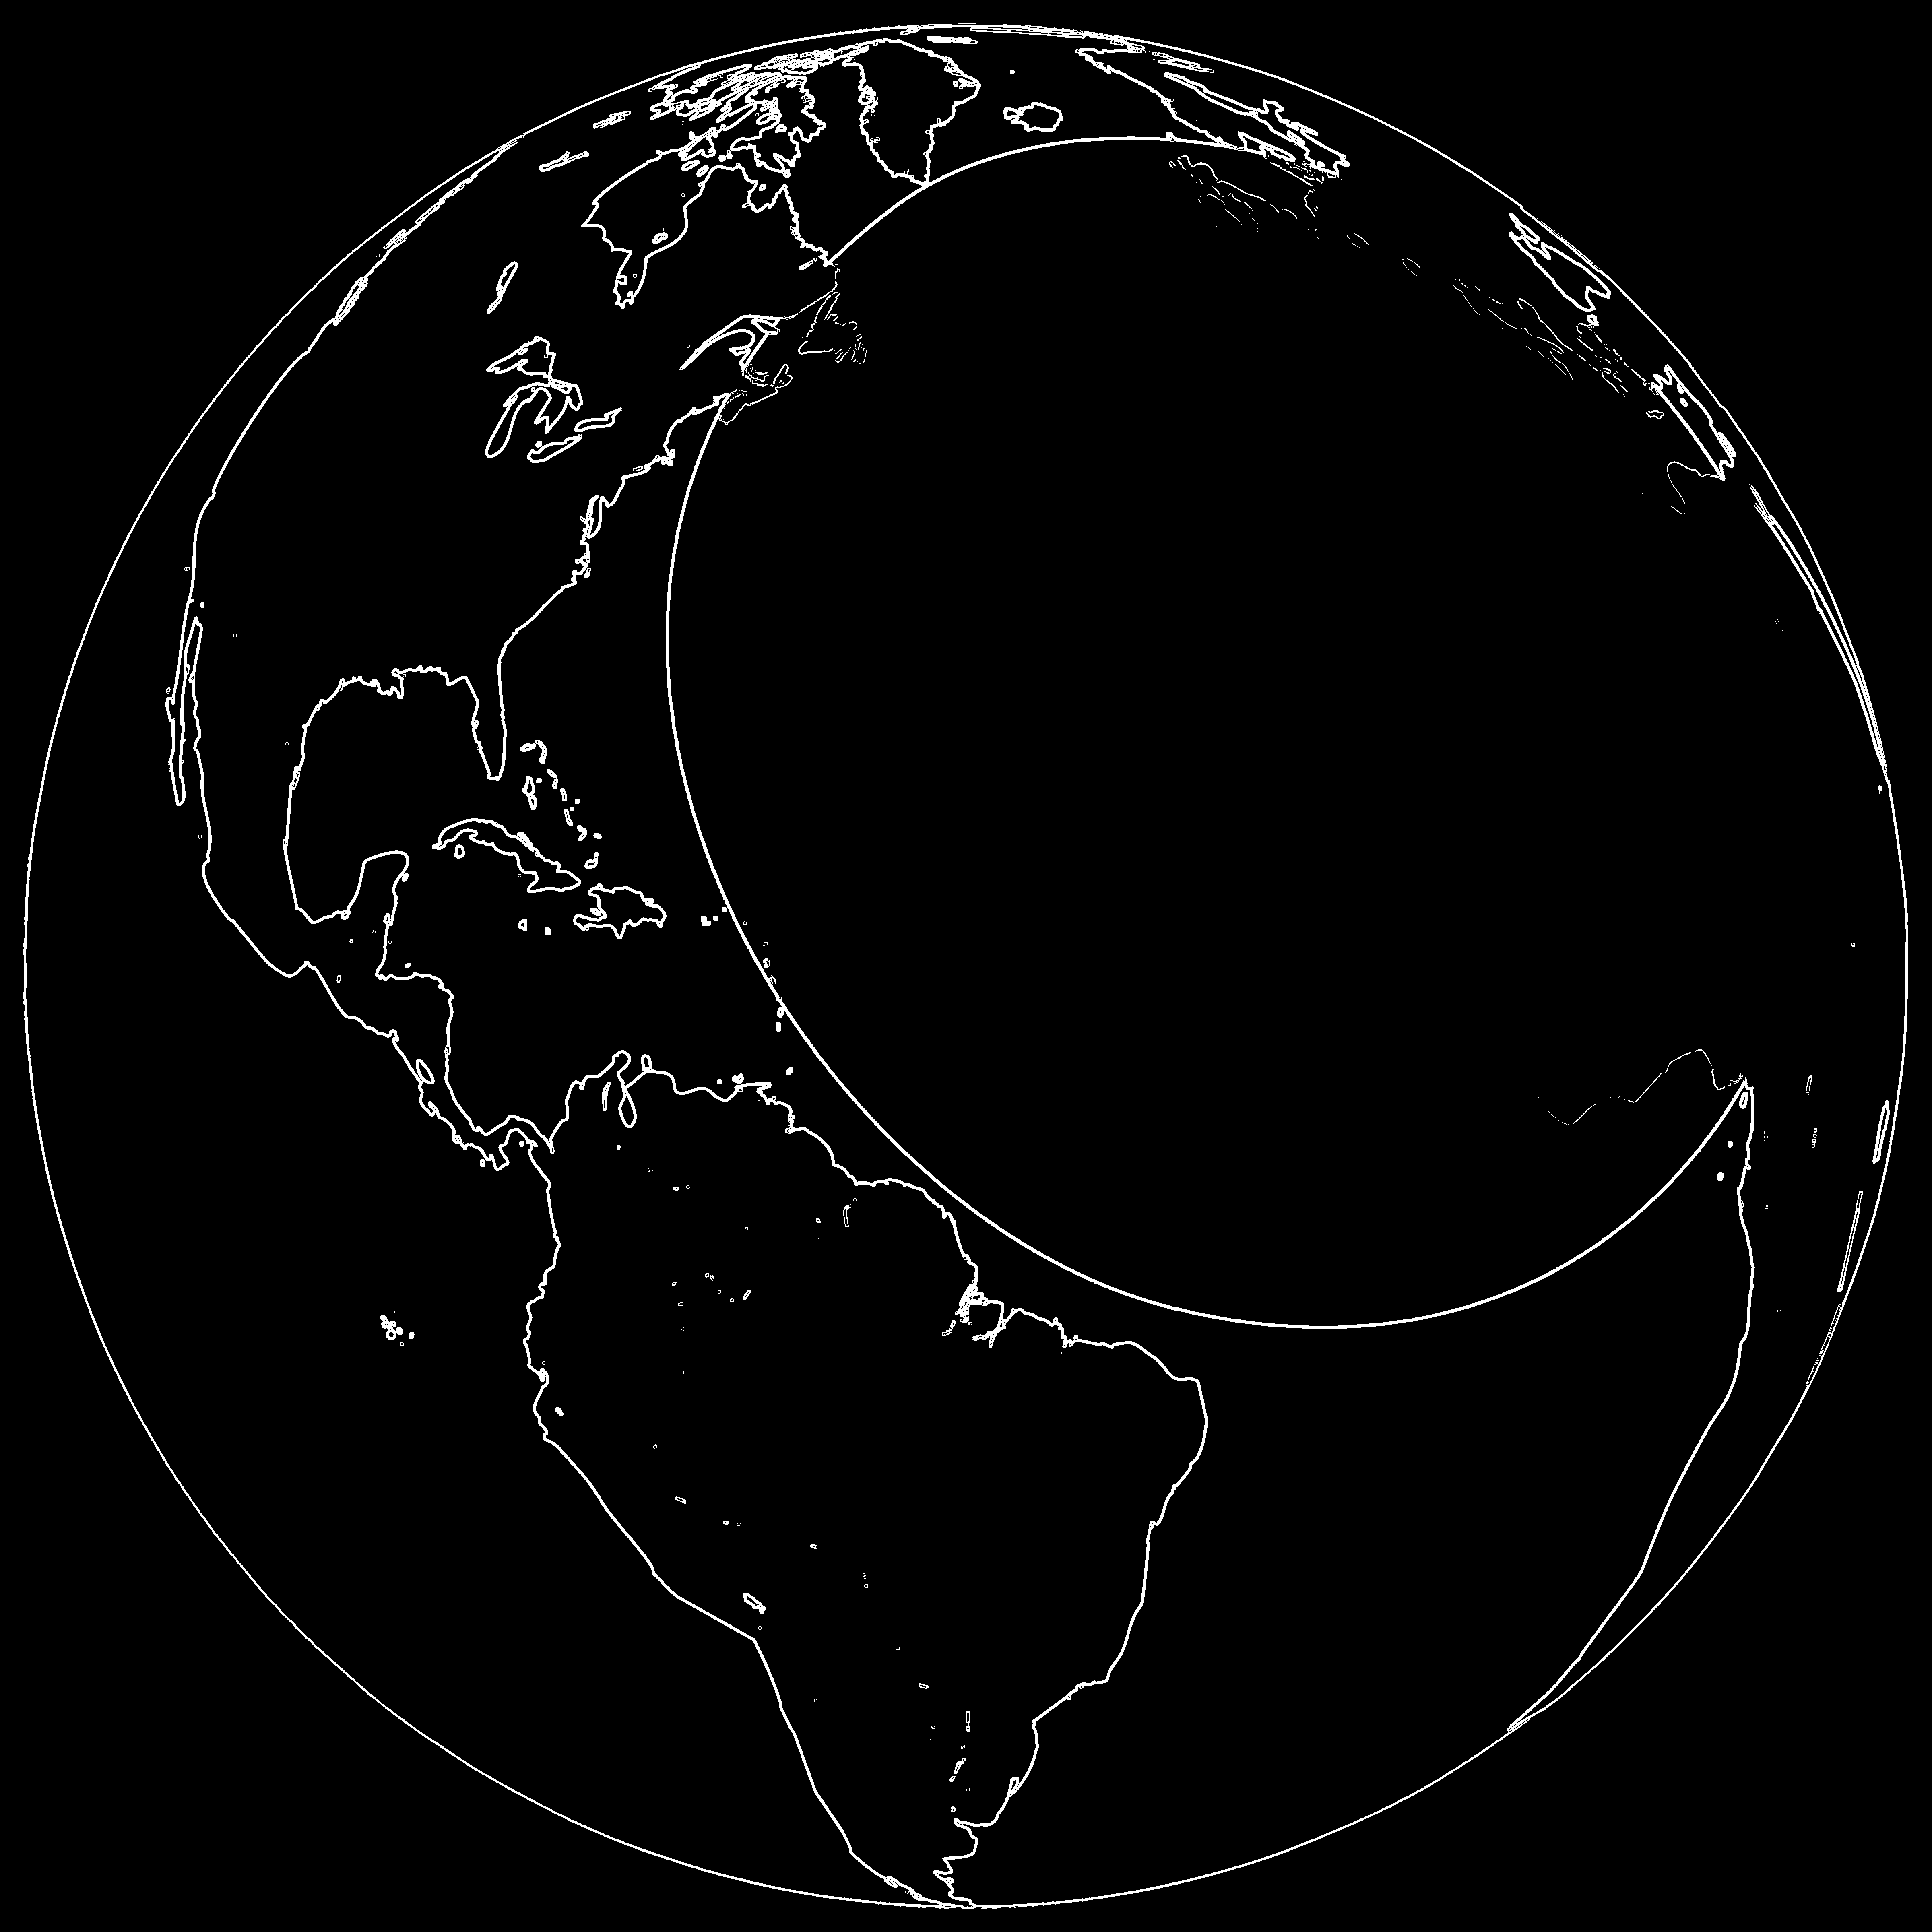
\includegraphics[scale=0.1]{earth_orig.png}
\end{figure}
\begin{figure}[H]
  \caption{Optimized Code Earth}
  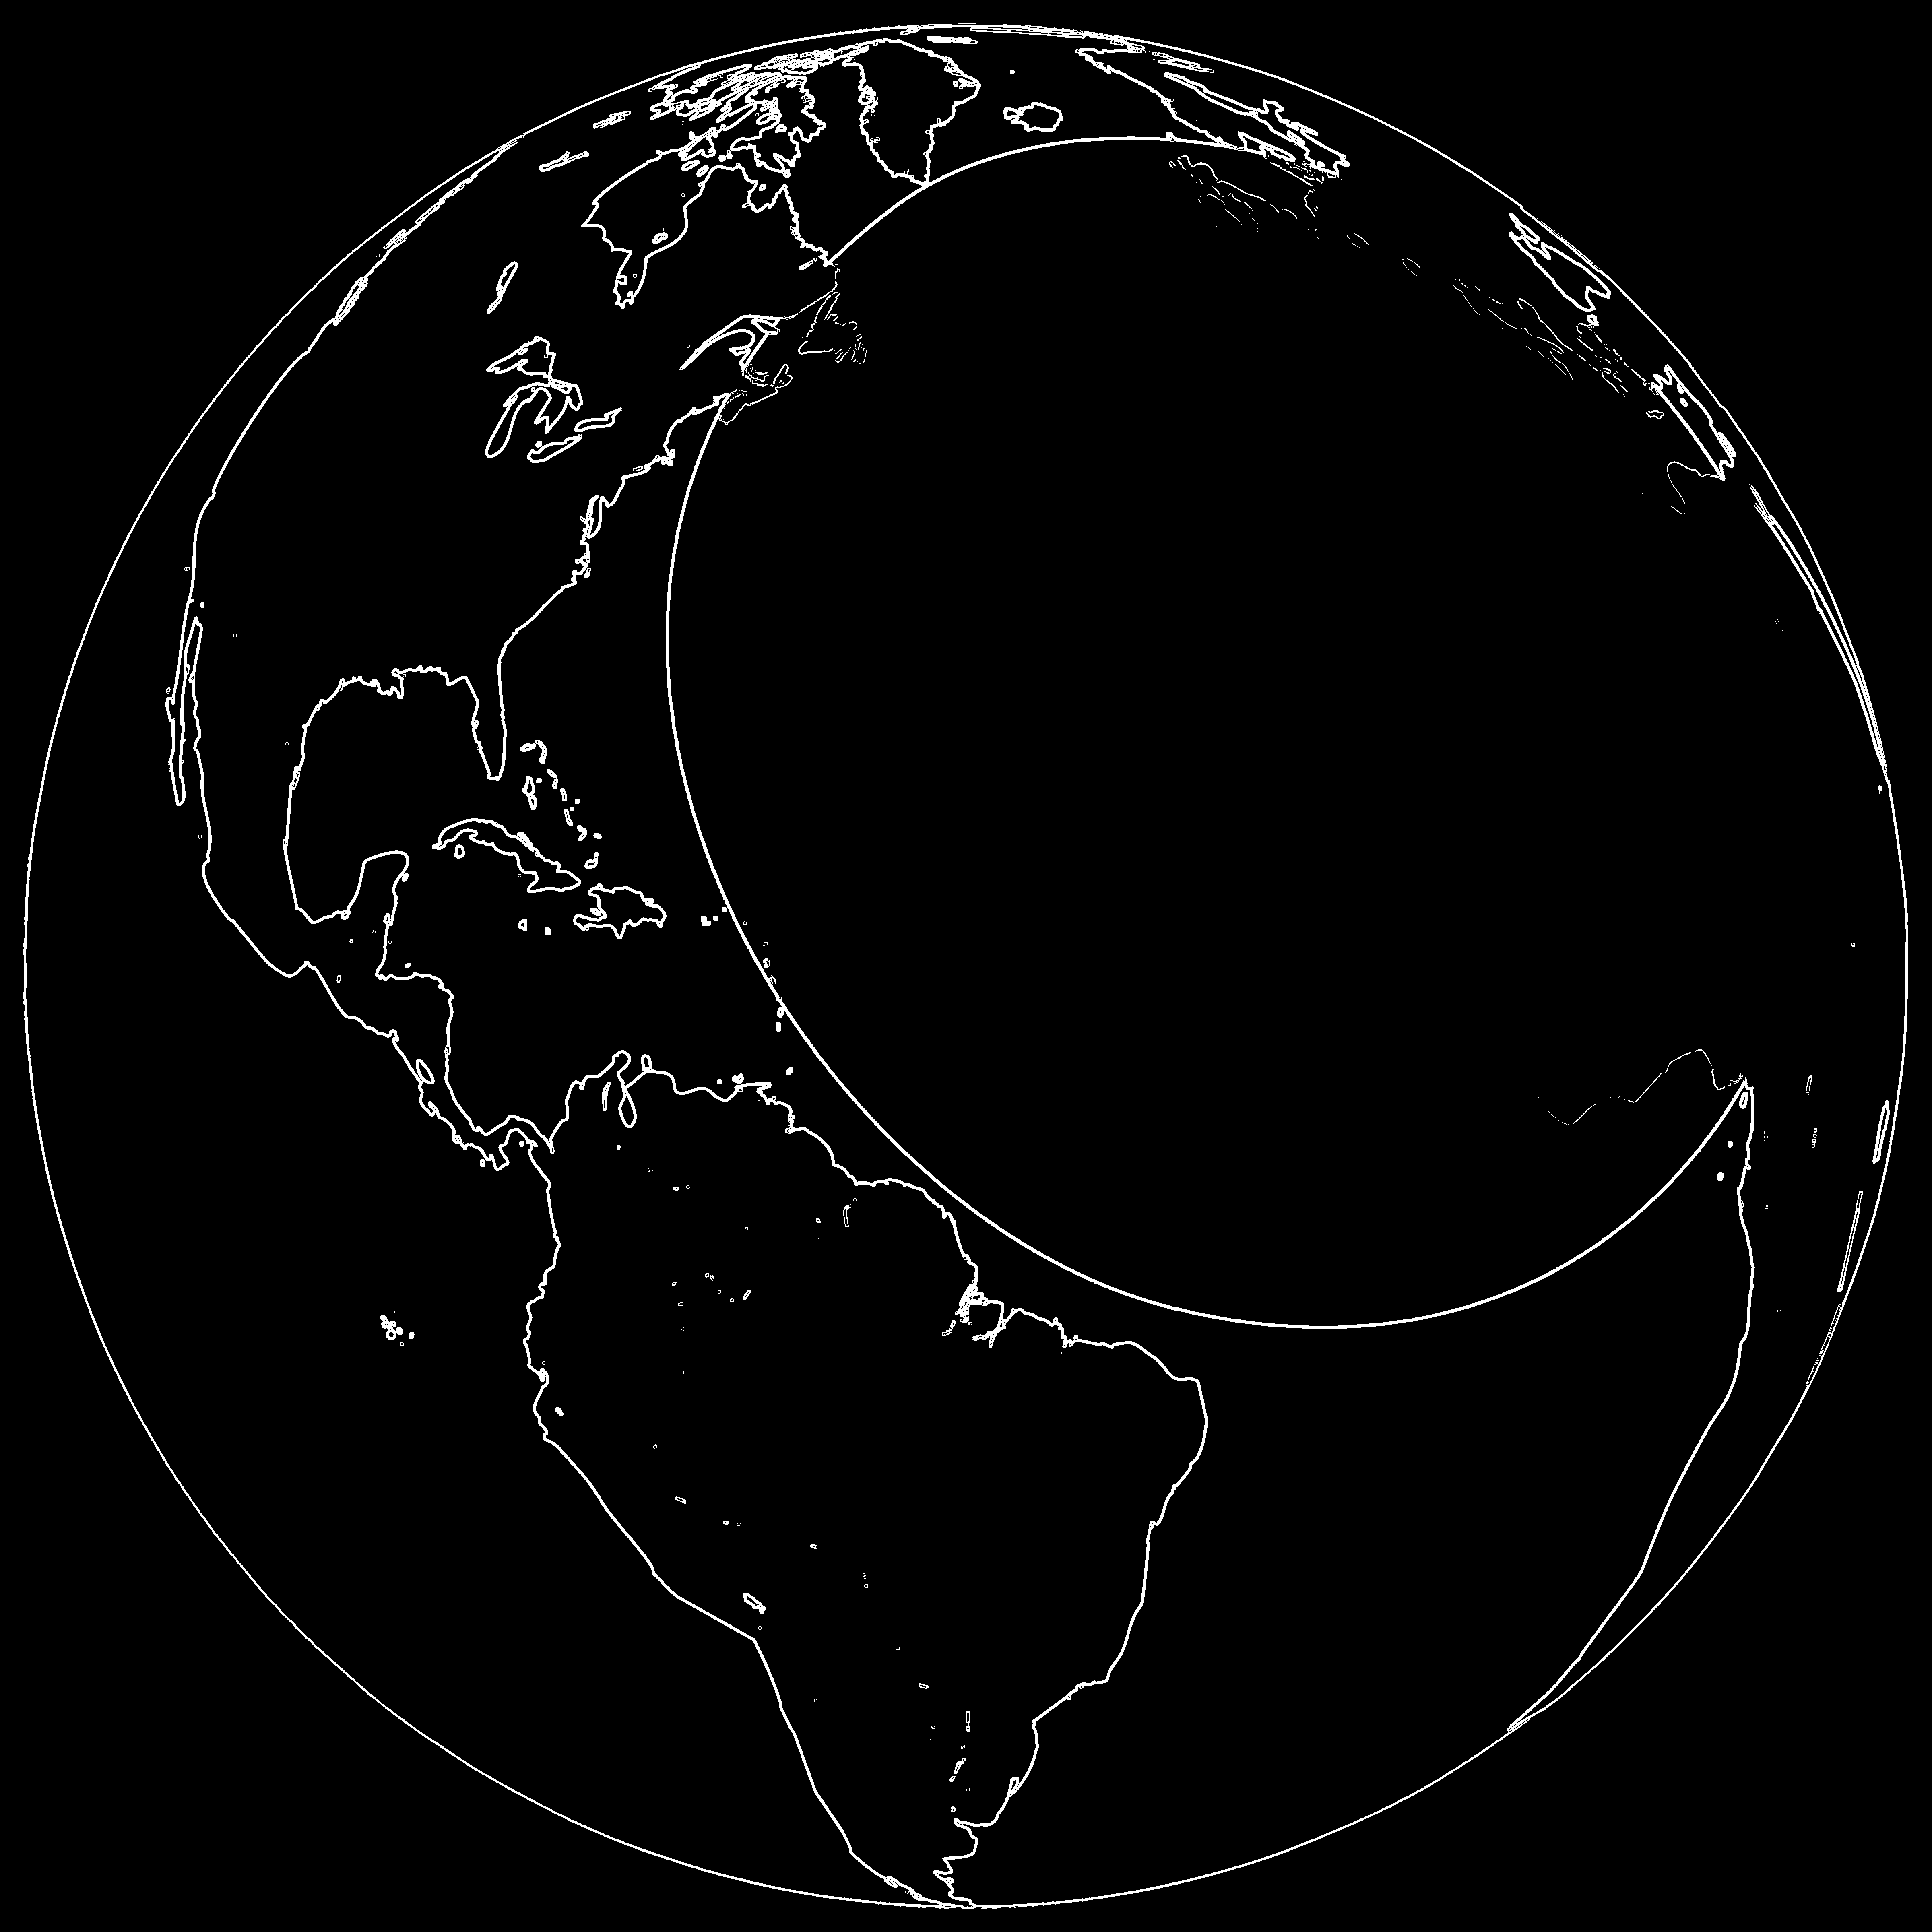
\includegraphics[scale=0.1]{earth_fast.png}
\end{figure}
\begin{figure}[H]
  \caption{Parallel Code Earth}
  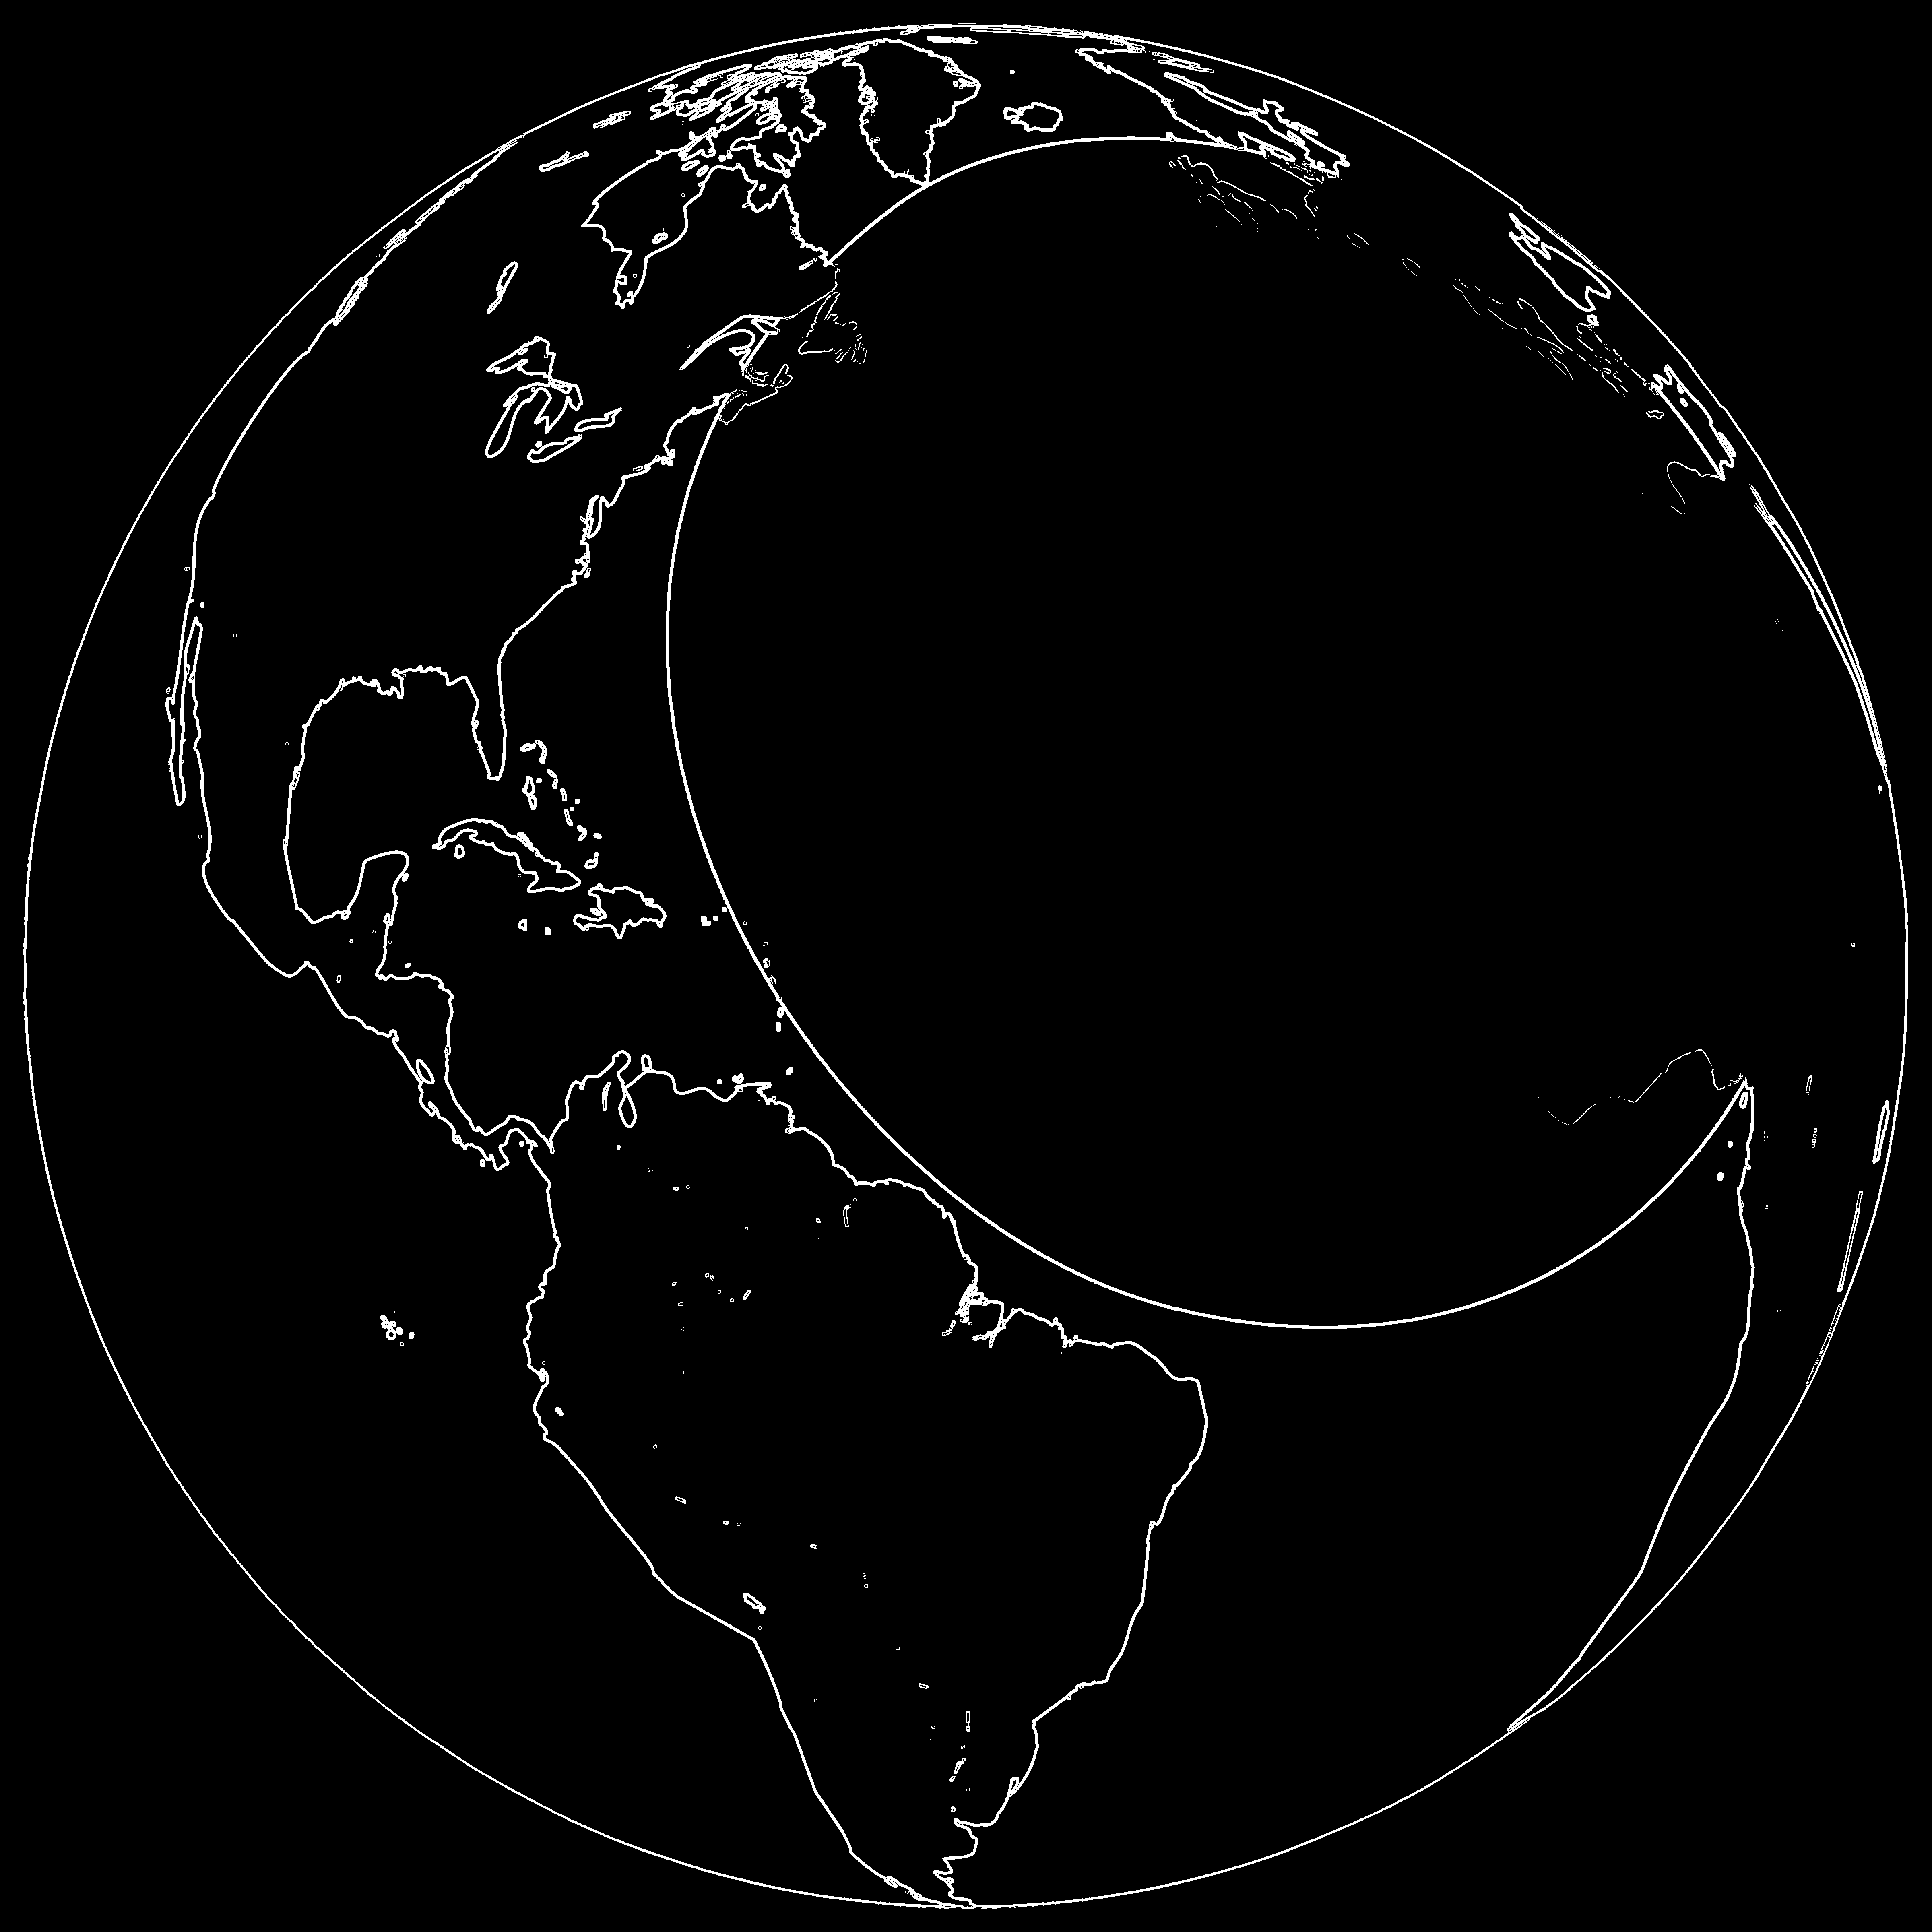
\includegraphics[scale=0.1]{earth_omp.png}
\end{figure}

My key takeaways involve both benchmarking and parallelizing code.  First, I have learned that benchmarking can be a bit tricky if your runtime is too small.  When testing the loop orders, I couldn't see improvements because the program was too quick.  I now know to pick inputs that give at least a few seconds of runtime.  My next key takewaway is that parallelizing code does not need to be a monumental task.  Rather than analyzing the intracacies of the program to exploit every ounce of parallelization, three parallel for loops can result in a very noticeable speedup with very little time invested.  

\end{document}
